\documentclass[fleqn]{article}
\usepackage{graphicx}
\usepackage{polski}
\usepackage[utf8]{inputenc}
\usepackage{listings}
\usepackage{amsmath}
\usepackage{courier}
\usepackage{graphicx}
\usepackage[top=0.3in, bottom=0.8in, left=0.8in, right=0.8in, a5paper]{geometry}
\newcommand\numberthis{\addtocounter{equation}{1}\tag{\theequation}}
\renewcommand{\familydefault}{\sfdefault}

\usepackage{listings}
\usepackage{color}
 
\definecolor{codegreen}{rgb}{0,0.6,0}
\definecolor{codegray}{rgb}{0.5,0.5,0.5}
\definecolor{codepurple}{rgb}{0.58,0,0.82}
\definecolor{backcolour}{rgb}{0.95,0.95,0.92}
 
\lstdefinestyle{mystyle}{
    commentstyle=\color{codegreen},
    keywordstyle=\color{magenta},
    numberstyle=\tiny\color{codegreen},
    stringstyle=\color{codepurple},
    basicstyle=\footnotesize,
    breakatwhitespace=false,         
    breaklines=true,                 
    captionpos=b,                    
    keepspaces=true,                 
    numbers=left,                    
    numbersep=5pt,                  
    showspaces=false,                
    showstringspaces=false,
    showtabs=false,                  
    tabsize=2
}
 
\lstset{style=mystyle}


\usepackage{color}
\color{white}
\pagecolor{black}

\begin{document}

\title{Sieci neuronowe}
\author{Szymon Bugaj}

\maketitle

\begin{abstract}
Sprawozdanie z laboratorium poświęconego sieciom neuronowym z przedmiotu ROB (Rozpoznawanie obrazów).
\end{abstract}

\section{Szczegóły dotyczące uczenia}
Zaimplementowany został perceptron wielowarstwowy z jedną warstwą ukrytą.
Użyta funkcja aktywacji to funkcja sigmoidalna. Przyjęte oznaczenia zgadzając się z tymi użytymi w wykładzie. Ponadto $g$ oznacza funkcję aktywacji dla warstw ukrytych, $o$ oznacza funkcję aktywacji dla warstwy wyjściowej. W funkcji $learnMLP$ brakuje możliwości wpisania pochodnych funkcji g, o - tym samym ma sens tylko dla funkcji sigmoidalnej.

Stała uczenia oznaczona jest literką $K$ i nie zmienia się podczas uczenia.
W warstwie ukrytej znajduje się 300 neuronów. Wagi początkowe są losowane w zależności od liczby neuronów w warstwie poprzedniej i aktualnej.

Algorytm jest zatrzymywany jeżeli przez 10 iteracji najlepszy wynik na zbiorze walidacyjnym nie został polepszony. Ostateczny model to ten, który dawał najlepszy wynik.

\begin{minipage}{\linewidth}
\begin {lstlisting}[language=Matlab]
g = @sigmoid
o = @sigmoid
N_y = 300
K_b = 0.01

function y = sigmoid(x)
	y = 2./(1+exp(-1 .* x))-1;
    
function weights = randWeights(N_h_prev, N_h)
	weights = (rand(N_h_prev,N_h)-0.5)* ...
        2*sqrt(6)/sqrt(N_h_prev+N_h);
	weights(N_h_prev, :) = 0;
\end{lstlisting}
\end{minipage}


\section{Rezultaty}
Podzieliłem oryginalny zbiór uczący na dwa podzbiory: nowy uczący i walidacyjny (50000 próbek i 10000 próbek). Ostateczny rezultat optymalizacji sprawdzany był na oryginalnym zbiorze testującym.

Ciekawym jest uzyskanie lepszego wynika na zbiorze testowym niż na zbiorze walidacyjnym ($1.95\%$ i $2.06\%$).

Uczenie trwało 42 minuty, odbyło się 58 iteracji.

Wykres przedstawia błąd walidacyjny w zależności od iteracji.

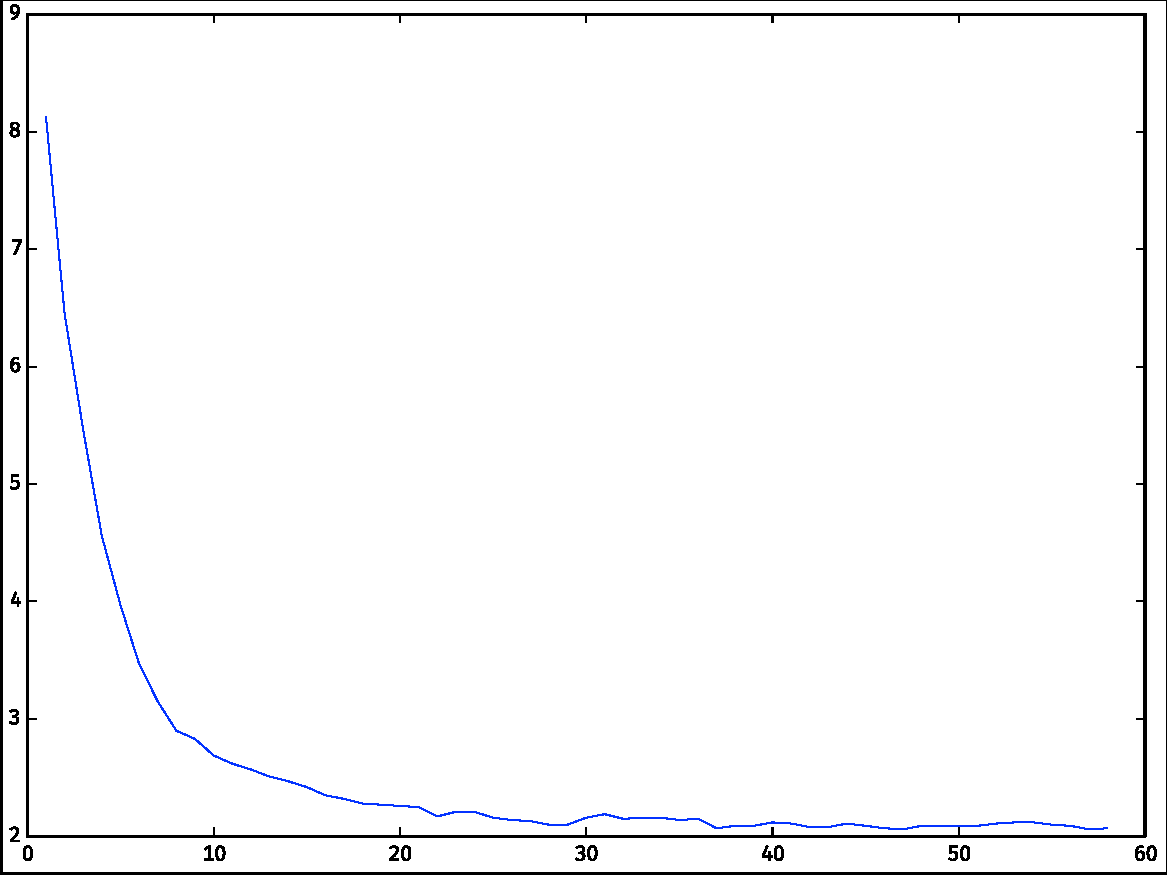
\includegraphics[width=10cm, height=7cm]{figure1.pdf}


\section{Modyfikacje}
Niestety nie mam obecnie czasu na zmiany.
Zmiany, które bym zaimplementował to: zmiana funkcji kary na softmax, podawanie próbek z prawdopodobieństwem proporcjonalnym do ostatnio uzyskanej funkcji kary (np po 5 iteracjach standardowych) tak by te gorzej klasyfikowane były częsciej podawane do sieci.


\end{document}